% !TeX root = ../main.tex
% 原始章节：09-test-and-show.Rmd

\chapter{回片测试与系统演示}\label{chap:09-test-and-show}

\section{芯片封装}\label{sec:09-test-and-show-001}

在LainChip流片过程中我们向封装公司提供了如下信息：

\begin{itemize}
\item
  芯片基本信息（主要参考晶圆厂给出的流片工艺信息）：

  \begin{longtable}[]{@{}
    >{\raggedright\arraybackslash}p{(\linewidth - 2\tabcolsep) * \real{0.5729}}
    >{\raggedright\arraybackslash}p{(\linewidth - 2\tabcolsep) * \real{0.4271}}@{}}
  \toprule\noalign{}
  \begin{minipage}[b]{\linewidth}\raggedright
  项目
  \end{minipage} & \begin{minipage}[b]{\linewidth}\raggedright
  参数
  \end{minipage} \\
  \midrule\noalign{}
  \endhead
  \bottomrule\noalign{}
  \endlastfoot
  来料方式：晶圆/蓝膜/裸片 & 晶元 \\
  是否需要划片（*） & 不需要 \\
  wafer尺寸（*） & 8 inch \\
  wafer形式【单芯full mask、MPW、MTK、其它】 & MPW \\
  wafer或者die材质【Low-k、锗硅、砷化镓等】 & 普通cmos锗硅 \\
  背面金属化 & （*）无； （ ）有：材料\_\_\_\_\_\_\_\_\_\_\_\_ \\
  圆片/Die来料厚度（*） & 12mil \\
  减薄厚度（*） & （*）厂家标准； （ ）其他\_\_\_\_\_\_\_\_\_\_\_\_ \\
  芯片名称 & LainChip \\
  芯片尺寸（含划片槽）（*） & 4956 * 4956 \\
  划片槽宽度Scribe Line(um) & 80 \\
  Chip Logo/ID坐标或特征点标识【判断装片方向用】【必填】 & 3146, 4819处文字：BUAA SCSE \\
  Pad（坐标）与 封装Pin对应关系（*） & 需提供Pad XY坐标绘制封装图纸 \\
  Opening Pad size: & \\
  PAD最小间距 & \\
  PAD最小尺寸（*） & 45*45um \\
  铝层厚度（顶层）（*） & 6 层金属；顶层金属厚度\textbf{9.825kA} \\
  铝层成分及含量（*） & \\
  是否BOAC(CUP)（*） & \\
  封装外型POD(*) & LQFP176 \\
  封装数量 & 50 \\
  金线/铜线 *线径？（*） & 20um金线 \\
  导电胶/绝缘胶？（*） & 导电胶 \\
  正印内容（*） & \\
  正印内容【*带图案，需提供Cad文件】 & \\
  \end{longtable}
\item
  Pab与Pin对应关系（该映射关系一般由芯片后端人员给出）：

  \begin{longtable}[]{@{}
    >{\raggedright\arraybackslash}p{(\linewidth - 10\tabcolsep) * \real{0.1833}}
    >{\raggedright\arraybackslash}p{(\linewidth - 10\tabcolsep) * \real{0.1833}}
    >{\raggedright\arraybackslash}p{(\linewidth - 10\tabcolsep) * \real{0.2500}}
    >{\raggedright\arraybackslash}p{(\linewidth - 10\tabcolsep) * \real{0.1167}}
    >{\raggedright\arraybackslash}p{(\linewidth - 10\tabcolsep) * \real{0.2000}}
    >{\raggedright\arraybackslash}p{(\linewidth - 10\tabcolsep) * \real{0.0667}}@{}}
  \toprule\noalign{}
  \begin{minipage}[b]{\linewidth}\raggedright
  封装【Pin】
  \end{minipage} & \begin{minipage}[b]{\linewidth}\raggedright
  芯片【Pad】
  \end{minipage} & \begin{minipage}[b]{\linewidth}\raggedright
  Location（X,Y）
  \end{minipage} & \begin{minipage}[b]{\linewidth}\raggedright
  \end{minipage} & \begin{minipage}[b]{\linewidth}\raggedright
  备注
  \end{minipage} & \begin{minipage}[b]{\linewidth}\raggedright
  \end{minipage} \\
  \midrule\noalign{}
  \endhead
  \bottomrule\noalign{}
  \endlastfoot
  Pin \# & Pad \# & X & Y & 名称 & \\
  1 & PADI45 & 278.66 & -35.415 & VSSIO & 3.3V \\
  2 & PADI45 & 375.32 & -35.415 & VDDIO & 3.3V \\
  3 & PADI45 & 471.98 & -35.415 & VSS & 1.8V \\
  4 & PADI45 & 568.64 & -35.415 & VDD & 1.8V \\
  5 & PADI45 & 665.3 & -35.415 & sdram\_DQ{[}19{]} & 3.3V \\
  6 & PADI45 & 761.96 & -35.415 & sdram\_DQ{[}18{]} & 3.3V \\
  7 & PADI45 & 858.62 & -35.415 & sdram\_DQ{[}17{]} & 3.3V \\
  8 & PADI45 & 955.28 & -35.415 & sdram\_DQ{[}16{]} & 3.3V \\
  ··· & ··· & ··· & ··· & ··· & ··· \\
  176 & PADI45 & -35.415 & 364.72 & VSSIO & 3.3V \\
  \end{longtable}
\end{itemize}

以上信息主要目的是为读者建立流片封装过程中我们需要完成的工作的概念，实际封装过程需按照厂家要求填写表格，以具体情况为准。

\section{测试PCB设计与制作}\label{sec:09-test-and-show-002}

我们为芯片回片后的测试设计了专用的PCB平台，集成电源芯片、SDRAM内存、FLASH以及USB PHY等芯片运行所需的硬件资源。该PCB使用国产LCEDA软件设计，共6个板层，其中第1、3、4、6为信号层，第2层为地层，第5层为电源层。PCB搭载的硬件资源如图\ref{fig:09-pcb-struct}所示。

\begin{figure}[htbp]
  \centering
  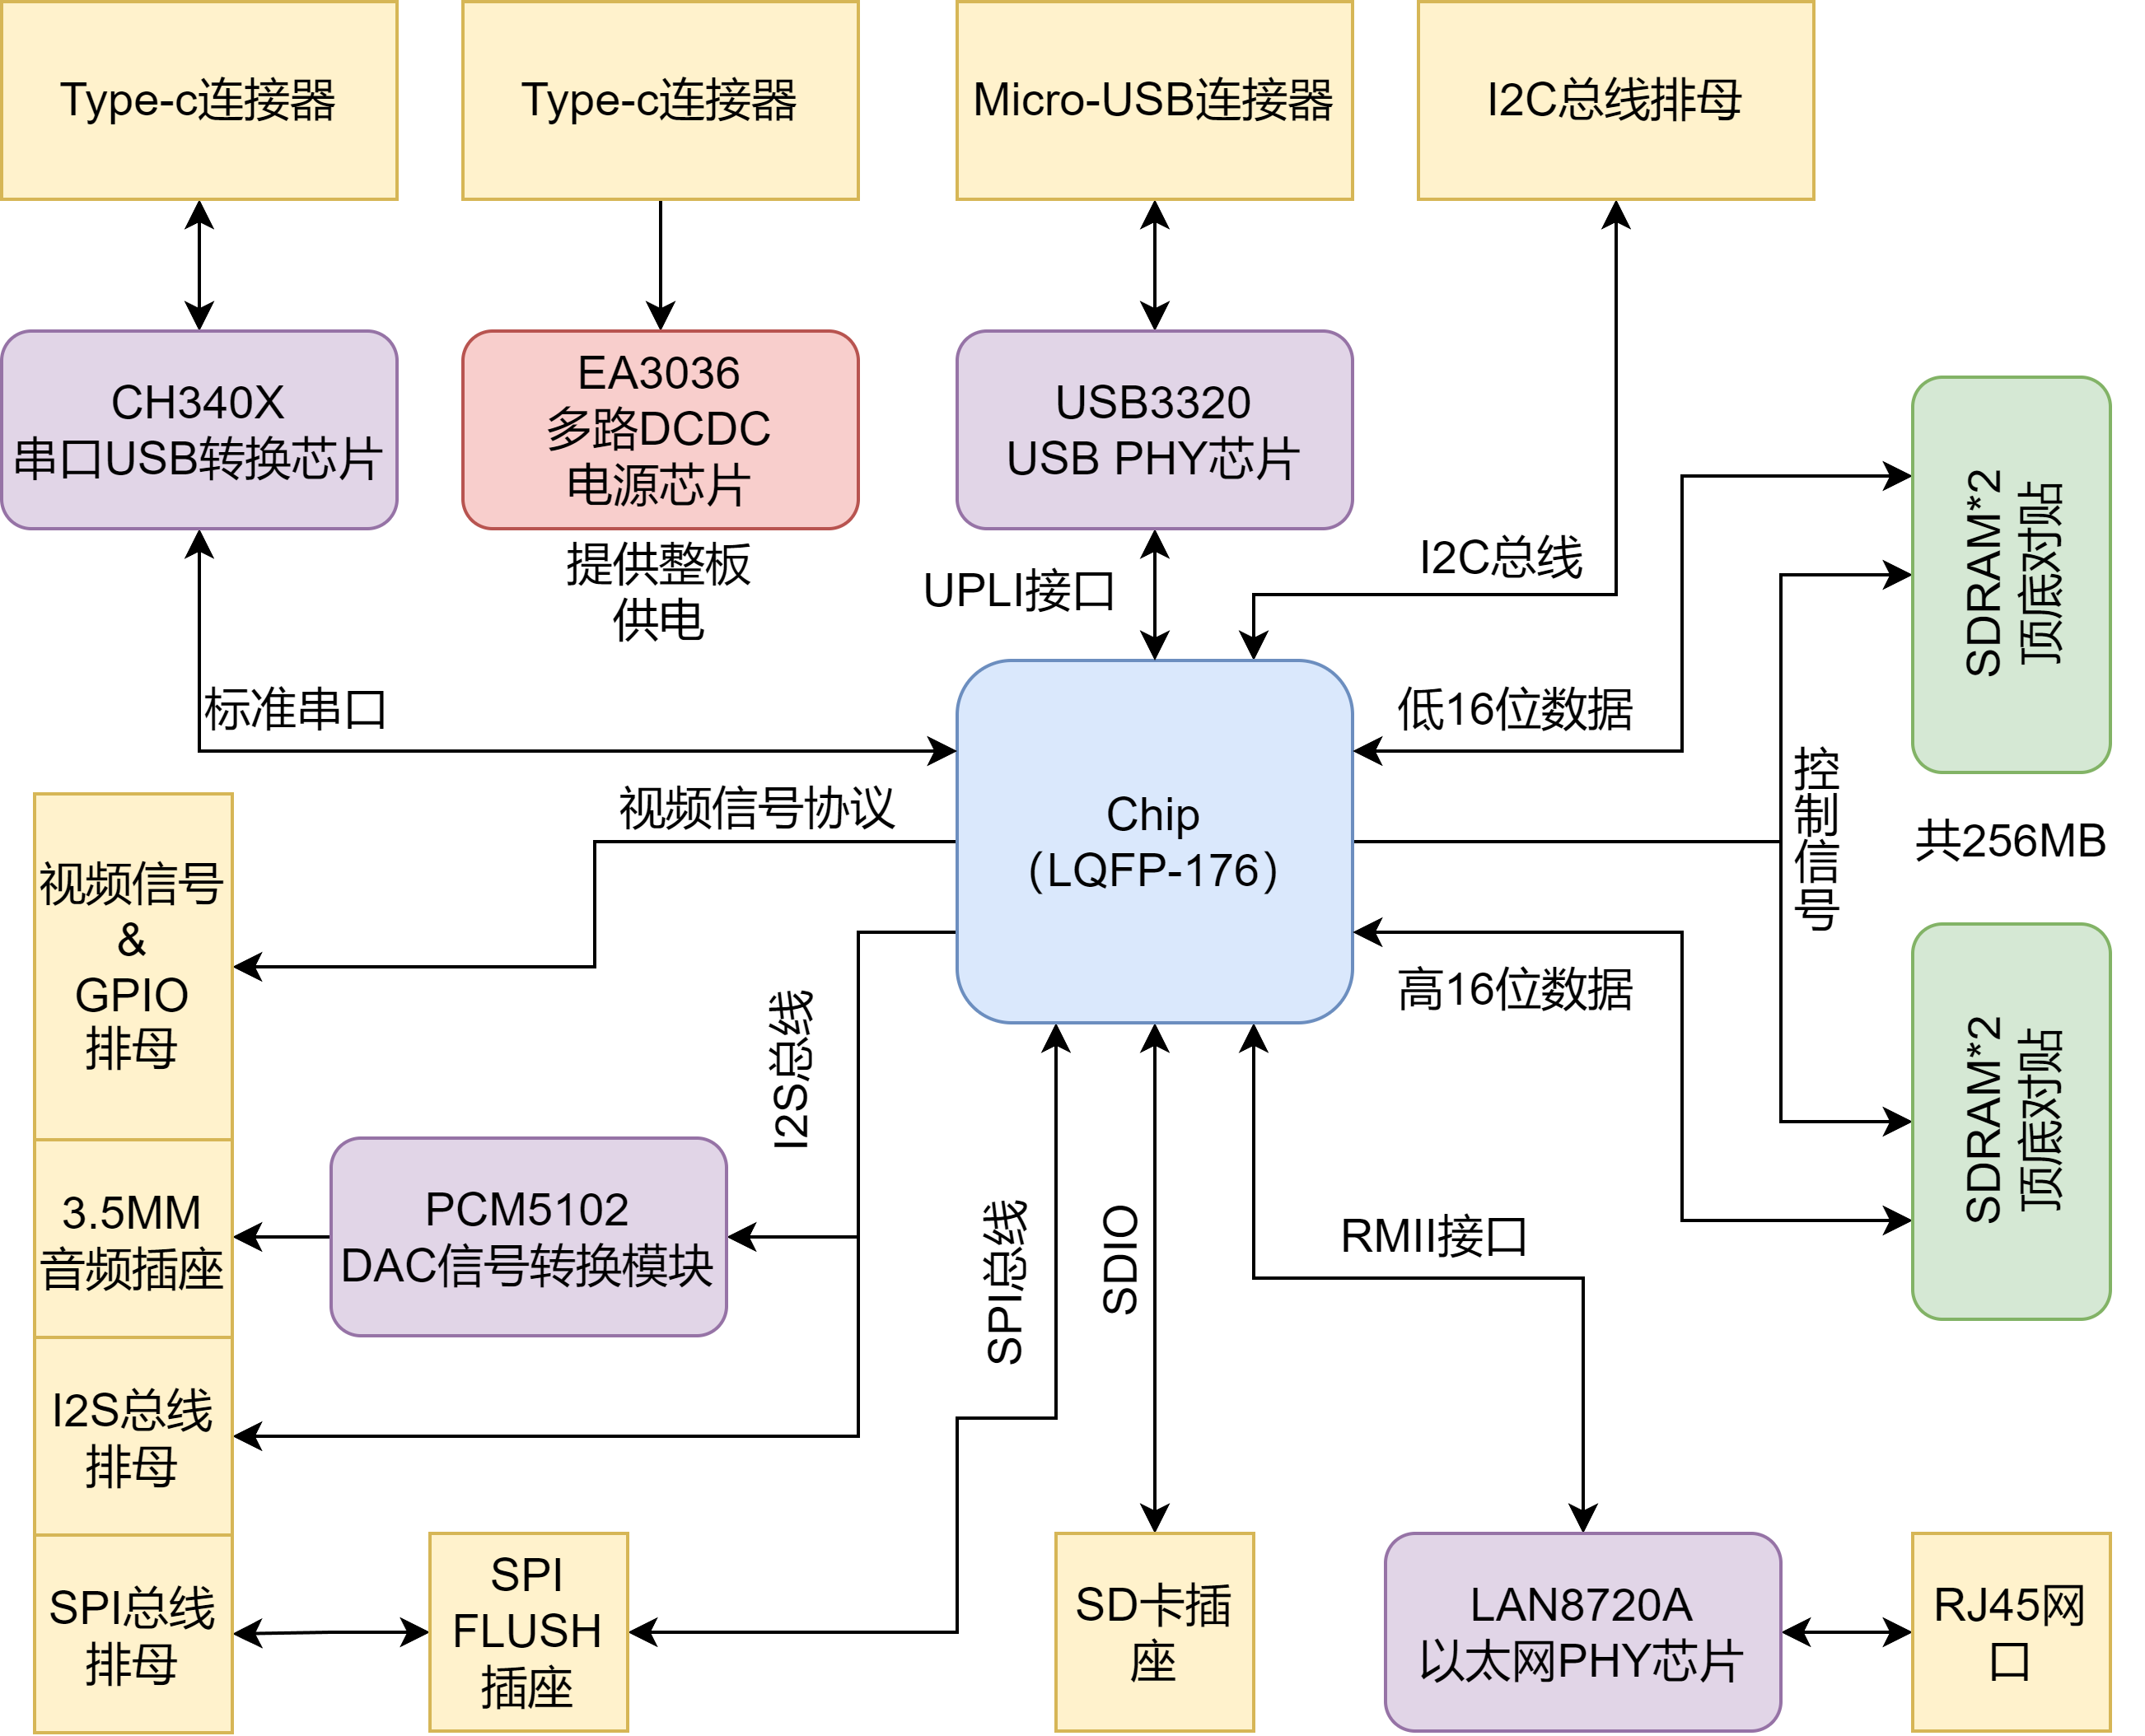
\includegraphics[width=0.75\linewidth]{assets/09/pcb-struct.png}
  \caption{PCB整体结构}
  \label{fig:09-pcb-struct}
\end{figure}

考虑到芯片及整板功耗较低，本设计供电方案选用Everanalog公司生产的EA3036电源芯片。EA3036是一款三路电源管理芯片，应用于直流5V供电或单节锂电池供电，内置三路同步电源调整模块，提供轻载高效模式，内置补偿电路，方便易用。电源电路原理图如图所示。其中3V3电源为板上外设提供供电，1V8电源主要为芯片内部电路提供供电，3V3\_CHIP电源专为芯片IO和内存芯片提供供电。

\begin{figure}[htbp]
  \centering
  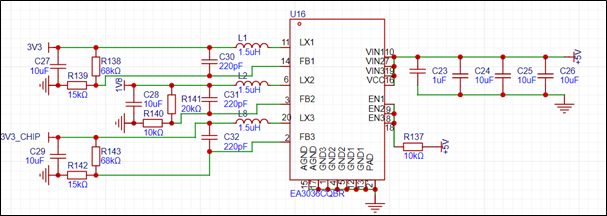
\includegraphics[width=1.0\linewidth]{assets/09/power.png}
  \caption{电源方案}
  \label{fig:09-power}
\end{figure}

内存芯片对于时序要求较高，设计过程中需要对走线长度进行控制，否则会影响信号完整性，产生数据错误。本文采用顶底对贴布局（在PCB顶层和底层重叠放置SDRAM芯片）并使用蛇形走线控制线长，所有SDRAM芯片的信号线线长度差值控制在5mm以内。图展示了本文其中两颗SDRAM芯片附近的走线情况。

\begin{figure}[htbp]
  \centering
  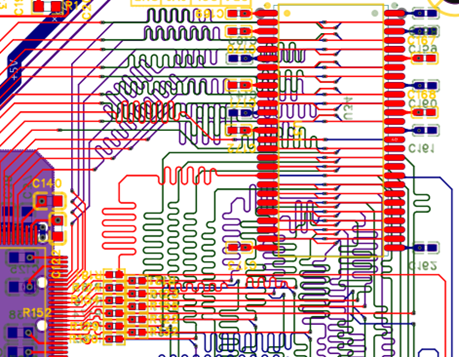
\includegraphics[width=0.5\linewidth]{assets/09/sdram.png}
  \caption{sdram走线}
  \label{fig:09-sdram}
\end{figure}

最终的测试板实物如图：

\begin{figure}[htbp]
  \centering
  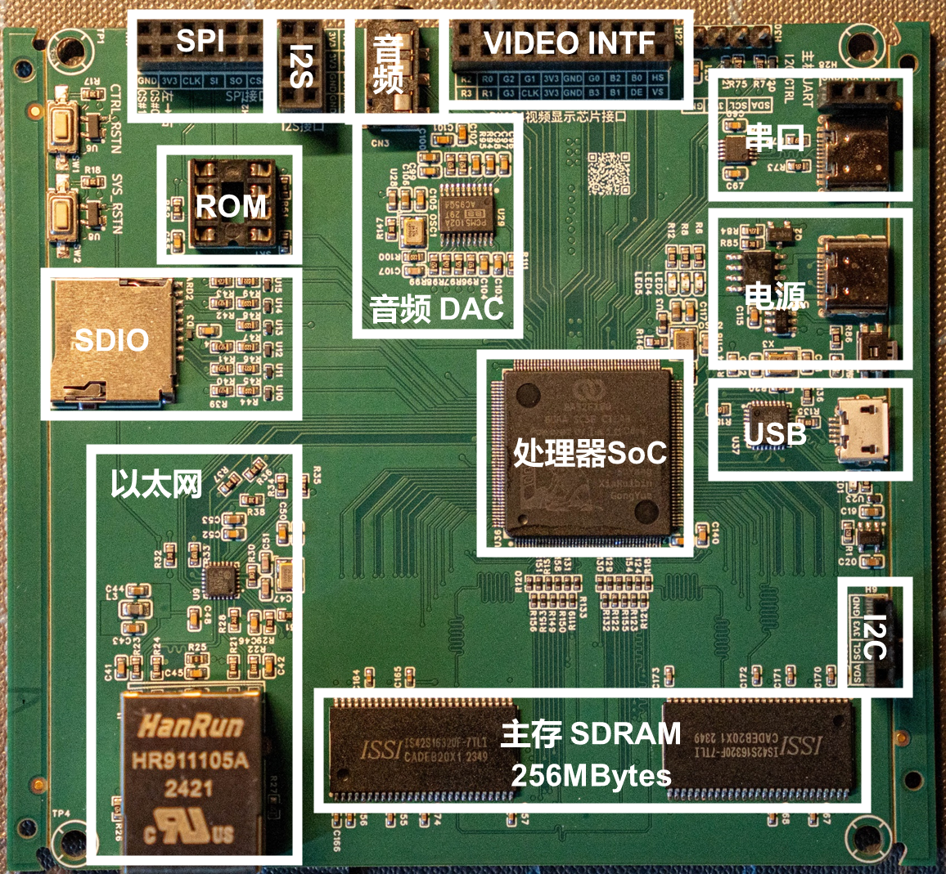
\includegraphics[width=0.75\linewidth]{assets/09/test-board.png}
  \caption{PCB实物图}
  \label{fig:09-test-board}
\end{figure}

我们推荐使用\href{https://pro.lceda.cn/}{立创EDA}设计PCB，该软件操作简单文档详实，同时与立创的整套服打通，方便元件的采购、PCB制作与SMT贴片。本文完整的PCB工程可点击\href{https://github.com/LainChip/LainBoard}{链接}浏览下载。

\section{芯片测试系统}\label{sec:09-test-and-show-003}

芯片回片后，我们在上小节开发板的基础上构建了一套基础的芯片测试系统。基于这套系统，我们对芯片的SPI、USB、网口、音视频接口等功能进行了完备的测试。我们设计的测试系统如图所示。

\begin{figure}[htbp]
  \centering
  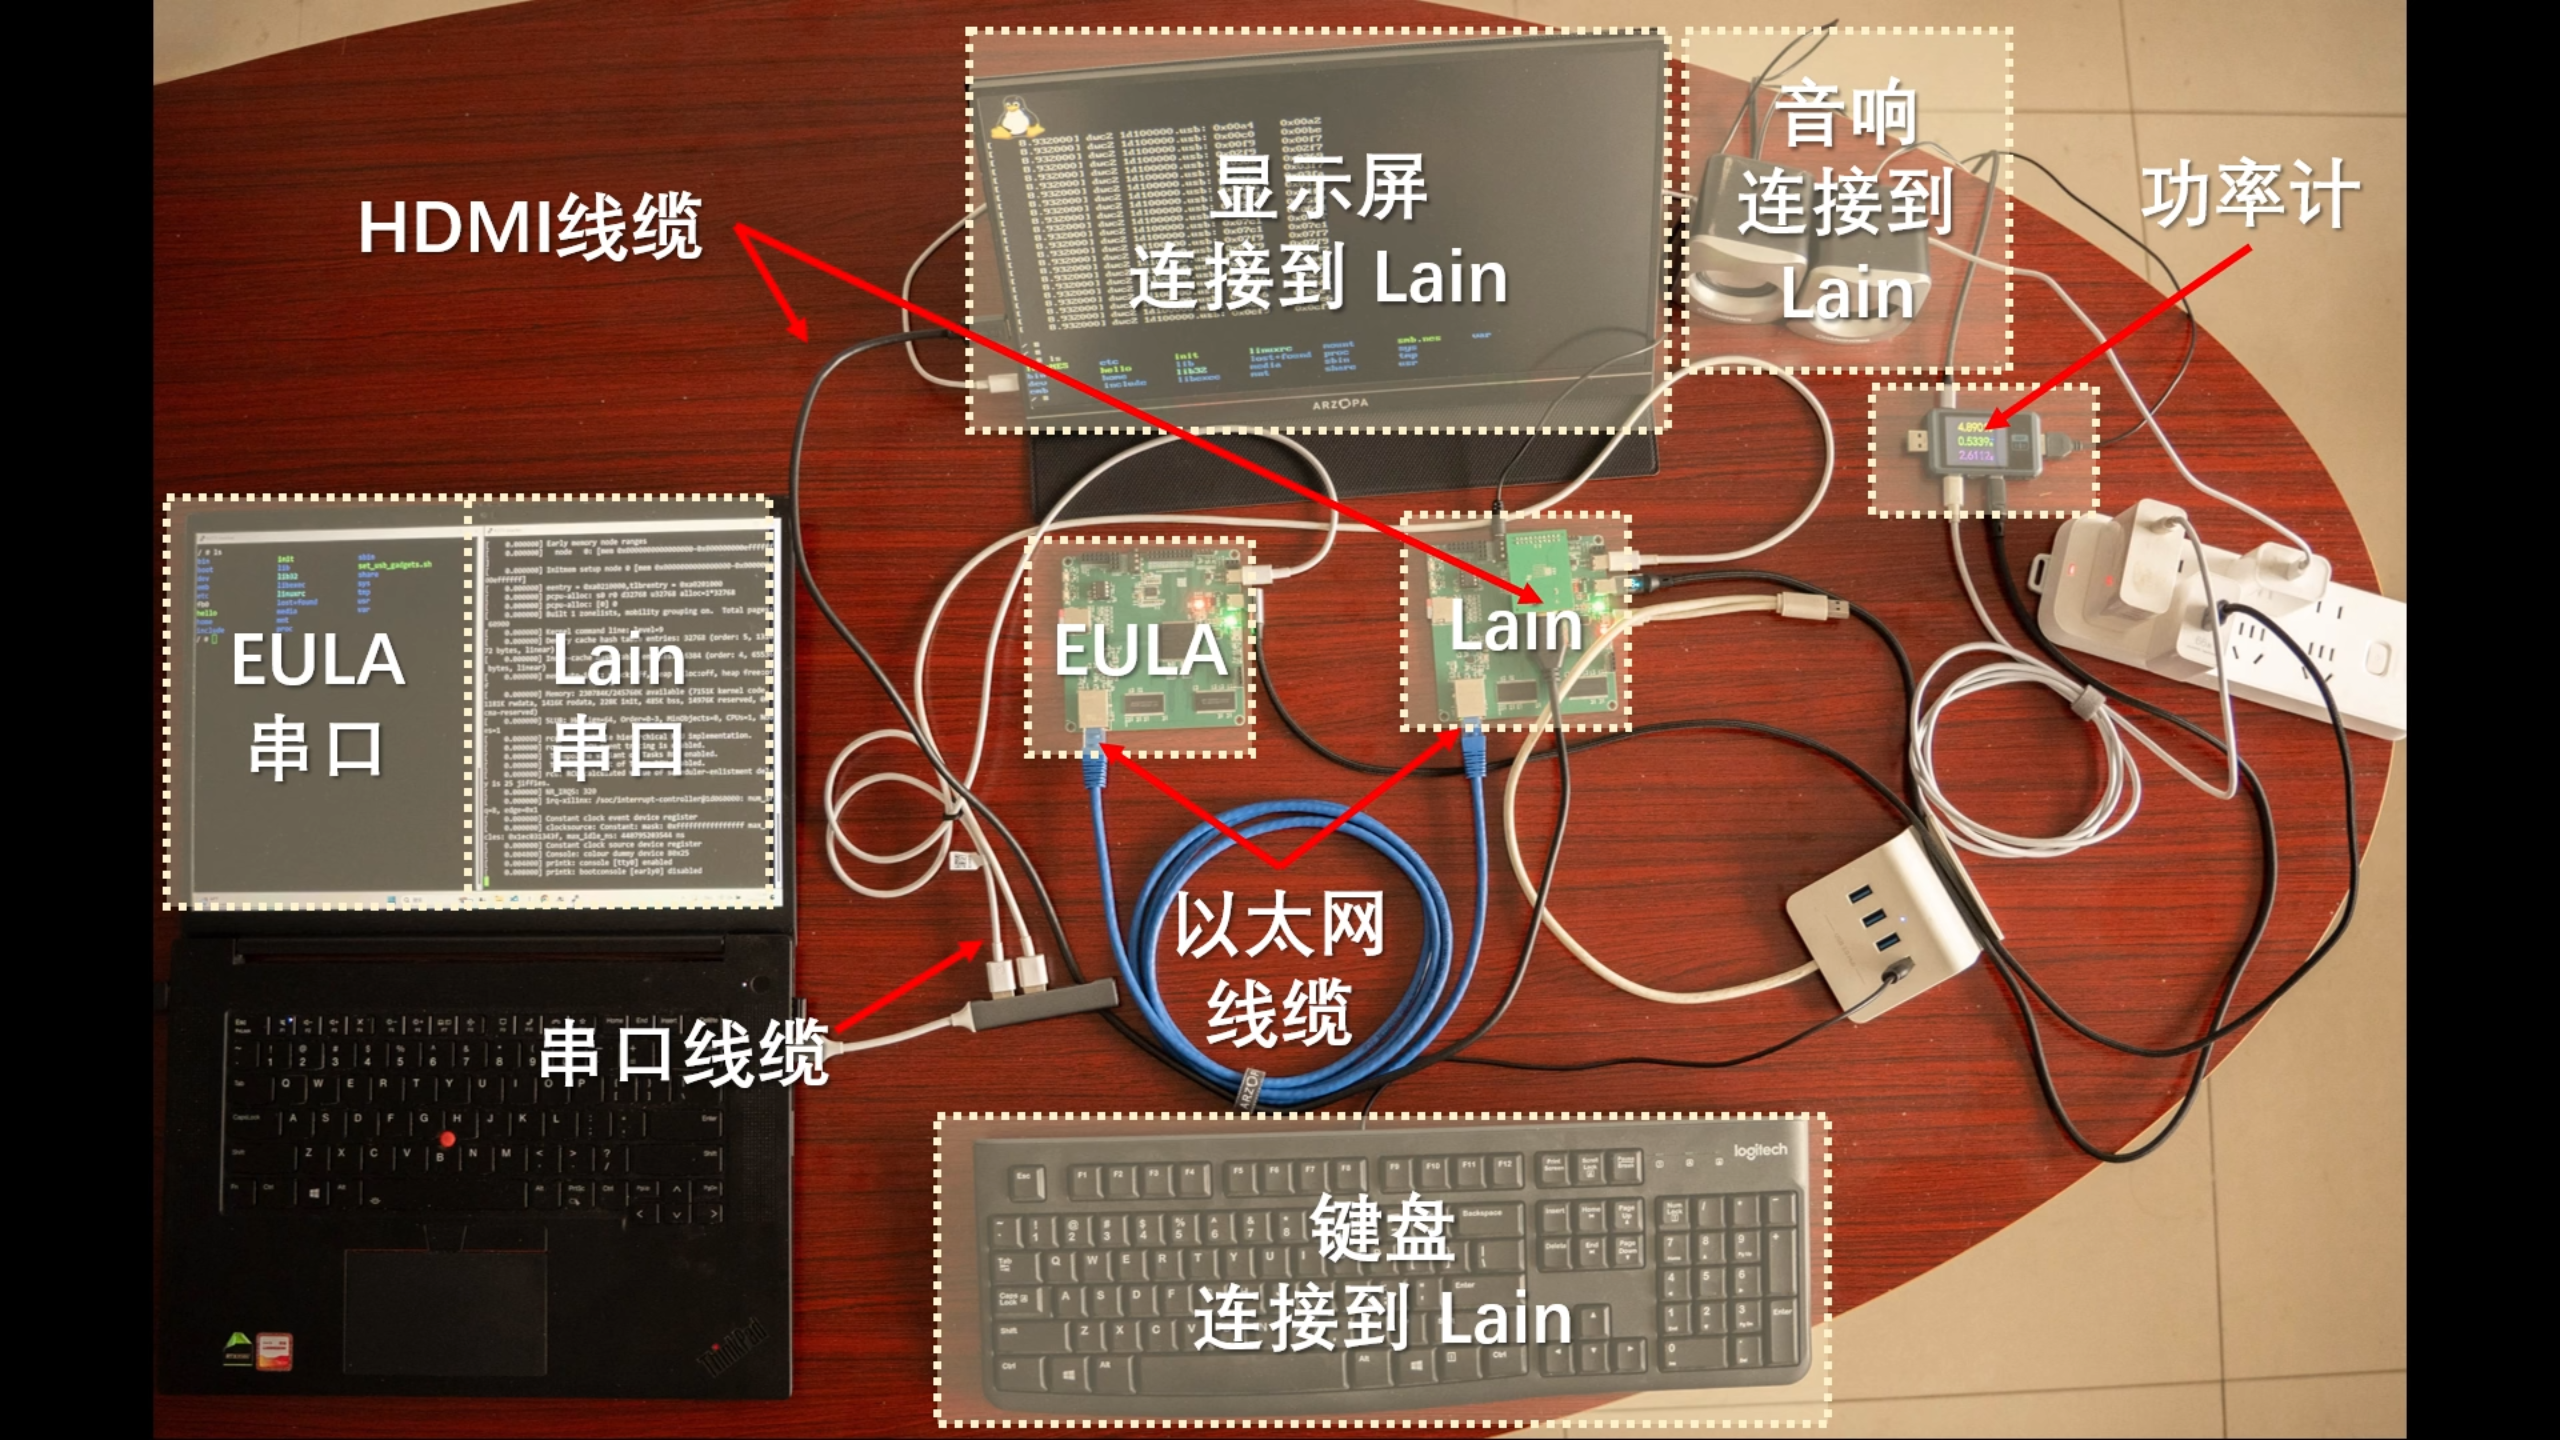
\includegraphics[width=1.0\linewidth]{assets/09/slt.png}
  \caption{测试系统}
  \label{fig:09-slt}
\end{figure}

该套测试系统的具体测试和运行效果可观看如下视频：\url{https://www.bilibili.com/video/BV1VUe8eHEgn}

\section{性能测试}\label{sec:09-test-and-show-004}

\section{功能演示}\label{sec:09-test-and-show-005}

\hspace{0pt} 功能演示是验证芯片是否按照设计规范工作的重要步骤。在这个阶段，通过一系列预定义的测试案例来展示芯片的基本功能和特性。 这些测试不仅验证了芯片的基本操作，还涉及到特殊情况和边缘情况，确保芯片在各种条件下都能可靠地工作。功能演示是客户和利益相关者评估产品性能的关键环节。

我们为回片后的 LainCore 及 EulaCore 构建了专用的演示程序，对片上搭载的大量硬件外设及处理器核心进行了综合配置使用，作为我们功能展示的应用。 具体来说，我们编写了视频播放软件，及幻灯片播放软件，可以支持简单格式视频及幻灯片的播放。 为了开发的便捷性，我们选用直接在 Uboot 中插入相关软件代码。Uboot 提供直接的软件交互环境和最小化的 C 运行时环境，及文件服务可以支持我们编写应用。

我们编写的裸机视频播放程序如下：

% 代码语言：BookC
\begin{CodeBlock}[language=BookC]
/*
 * (C) Copyright 2023
 * Wang Zhe, dofingert@gmail.com
 */

#include <common.h>
#include <command.h>
#include <mapmem.h>
#include <asm/cache.h>
#include <linux/bitops.h>

struct decode_ip_ctl
{
    volatile uint32_t ctrl;
    volatile uint32_t status;
    volatile uint32_t src;
    volatile uint32_t dst;
    volatile uint32_t stride;
    volatile uint32_t iocen;
};

struct i2s_ip_ctl
{
    volatile uint32_t version;         // 0x0 - 0x3
    volatile uint32_t conf;            // 0x4 - 0x7
    volatile uint32_t pad0[66];      // 0x8 - 0x10f
    volatile uint32_t mm2s_ctrl;       // 0x110
    volatile uint32_t mm2s_status;     // 0x114
    volatile uint32_t mm2s_multiplier; // 0x118
    volatile uint32_t mm2s_period;     // 0x11c
    volatile uint32_t mm2s_dmaaddr;    // 0x120
    volatile uint32_t mm2s_dmaaddr_msb; // 0x124
    volatile uint32_t mm2s_transfer_count; // 0x128
    volatile uint32_t pad1[6];             // 0x12c - 0x143
    volatile uint32_t mm2s_channel_offset; // 0x144
};

struct fb_ip_ctl
{
    volatile uint32_t conf;
    volatile uint32_t status;
    volatile uint32_t addr;
    volatile uint32_t length;
    volatile uint32_t hcfg[4];
    volatile uint32_t vcfg[4];
};

/*
    8M RESERVE;
    8M VBUF:
    |-------------------------|  8M == 0x0F80_0000 == 248M
    | Framebuffer             |
    |-------------------------|  6M
    | Framebuffer             |
    |-------------------------|  4M
    | Framebuffer             |
    |-------------------------|  2M
    | Framebuffer             |
    |-------------------------|  0M == 0x0F00_0000 == 240M
*/
// FRAMEBUFFER 必须 4k 对齐
static uint32_t frame_size_y, frame_size_x, dec_color_mode;
static uint32_t framebuffer_size = (2 * 1024 * 1024);
#define FRAMEBUFFER_START (0x0F000000)
/*
    File Format:

    |-------------------------|
    | BHeader (512 bytes)     |
    |-------------------------|
    | Video Frame + Pad       |
    |-------------------------|  x 128
    | Audio Frame + Pad       |
    |-------------------------|
    | BHeader (512 bytes)     |
    |-------------------------|
    | Video Frame + Pad       |
    |-------------------------|  x 128
    | Audio Frame + Pad       |
    |-------------------------|
*/
struct headerb
{
    uint32_t frame_size[128];
};
static int sample_perframe;
static int fps;
static struct i2s_ip_ctl *i2s_ctl;
static struct fb_ip_ctl  *fb_ctl;
static struct decode_ip_ctl *decode_ctl;
static uint32_t *ab_array[4];

static void fb_play_one_frame(uint32_t fbuf_ptr) {
    fb_ctl->addr = fbuf_ptr;
    fb_ctl->status = BIT(1);
}

static void open_i2s_device(void) {
    i2s_ctl->mm2s_ctrl = BIT(1);
    uint32_t iters=0;
    while(i2s_ctl->mm2s_ctrl & BIT(1)) {
        if((iters++) & 0xffff) {
            printf("Open I2S STUCK %x", i2s_ctl->mm2s_ctrl);
            i2s_ctl->mm2s_ctrl = 0;
        }
    }
    i2s_ctl->mm2s_ctrl = BIT(13) | (0x1 << 16) | (0x2 << 19);
    i2s_ctl->mm2s_multiplier = 512;
}

static void close_i2s_device(void) {
    i2s_ctl->mm2s_ctrl = BIT(1);
    uint32_t iters=0;
    while(i2s_ctl->mm2s_ctrl & BIT(1)){
        if((iters++) & 0xffff) {
            printf("Close I2S STUCK");
            i2s_ctl->mm2s_ctrl = 0;
        }
    }
    i2s_ctl->mm2s_ctrl = 0;
}

static void i2s_play_one_frame(uint32_t abuf_ptr) {
    i2s_ctl->mm2s_dmaaddr = abuf_ptr;
    i2s_ctl->mm2s_dmaaddr_msb = 0;
}

static int play_one_frame(int fb_num)
{
    uint32_t vbuf_ptr = FRAMEBUFFER_START + framebuffer_size * fb_num;
    uint32_t abuf_ptr = (uint32_t) ab_array[fb_num];
    i2s_play_one_frame(abuf_ptr);
    fb_play_one_frame(vbuf_ptr);
    return 0;
}

static uint32_t padding(uint32_t in)
{
    return ((in + 511) / 512) * 512;
}

static int decode_one_frame(int frame_size,
                            void *jpeg_file_ptr,
                            int fb_num)
{
    int vframe_size;
    vframe_size = frame_size;

    decode_ctl->ctrl = 0x40000000;

    // 配置 decode ip 的地址
    decode_ctl->src = ((uint32_t)jpeg_file_ptr) & 0x1fffffff;
    decode_ctl->dst = FRAMEBUFFER_START + framebuffer_size * fb_num;
    // FIXED 1280x720p @ 16bits, but resolution might be various.
    decode_ctl->stride = frame_size_x * (dec_color_mode ? 3 : 2); 
    // 配置开始 decode ip 的解码
    decode_ctl->iocen = 1 | ((dec_color_mode & 1) << 1); // 打开中断输出，清理旧的中断
    decode_ctl->ctrl  = 0x80000000 | vframe_size;

    // 音频数据指针写入到音频指针缓冲区
    ab_array[fb_num] = 
      (uint32_t *)(((uint32_t)(jpeg_file_ptr + padding(vframe_size))) & 0x1fffffff);
    return 0;
}

// return 0 on finish.
static int get_next_frame_ptr(int init, void **binary)
{
    static int sub_frame_cnt;
    static struct headerb *hdr_b;
    if(init) {
        sub_frame_cnt = 0;
        hdr_b = *binary;
        *binary += 512;
    } else {
        uint32_t aframe_size = padding(sample_perframe * 4);
        *binary += padding(hdr_b->frame_size[sub_frame_cnt++]) + aframe_size;
    }
    if(sub_frame_cnt >= 128) {
        sub_frame_cnt = 0;
        hdr_b = *binary;
        *binary += 512;
    }
    return hdr_b->frame_size[sub_frame_cnt];
}

static int wait_an_interrupt(int target_mask, int forever)
{
    uint32_t iters = 0;
    while(1) {
        uint32_t estate, irqs;
        asm volatile(
		"	csrrd	%0, 0x5\n"
		: "=r"(estate) :: "memory");
        irqs = (estate >> 4) & target_mask;
        if(irqs){
            return irqs;
        }

        iters++;
        if((iters & 0xfffff) == 0 && !forever) {
            printf("NIR%d,%x\n",iters, estate);
            return 0;
        }
    }
}

static int mediaplayer(void *binary)
{
    int decode_ptr = 0, play_ptr = 0, finish_flag = 0, fifo_size = 0, int_cnt = 0;
    int frame_size;
    // 初始化 I2S 控制器
    printf("offset of MM2S_CTRL is %x\n", 
           (uint32_t)(&i2s_ctl->mm2s_ctrl) - (uint32_t)i2s_ctl);
    open_i2s_device();
    // 先解码四帧填满
    for(int i = 0 ; i < 4 ; i++) {
        frame_size = get_next_frame_ptr(i == 0, &binary);
        if(frame_size == 0) {
            finish_flag = 1;
            break;
        }
        decode_one_frame(frame_size,binary,decode_ptr++);
        wait_an_interrupt(0x2, 1);
        decode_ptr &= 3;
        fifo_size++;
    }
    // 之后播放第一帧
    play_one_frame(play_ptr++);
    i2s_ctl->mm2s_period = (2 << 16) | (sample_perframe * 2);
    i2s_ctl->mm2s_ctrl = BIT(0) | BIT(13) | (0x1 << 16) | (0x2 << 19);
    i2s_ctl->mm2s_channel_offset = sample_perframe * 1;
    play_ptr &= 3;
    fifo_size --;
    // FIFO_SIZE == 3, FULL.
    uint32_t iter;
    // 开始轮询中断
    while(1) {
        if(finish_flag && fifo_size == 0) {
            printf("Play end!\n");
            break;
        } // 播放完成，退出
        int irq = wait_an_interrupt(0x3, 0);
        if(irq & 0x1) {
            if(fifo_size) {
                // I2S IRQ DRIVENED PLAY NEEDED
                i2s_ctl->mm2s_status = BIT(31); // DISABLE INTERRUPT
                while(1) {
                    uint32_t estate;
                    asm volatile(
                        "	csrrd	%0, 0x5\n"
                        : "=r"(estate) :: "memory");
                    if(!(estate & (0x1 << 4))) break;
                }
                if((int_cnt++) & 1) {
                    int_cnt &= 1;
                } else {// Dosen't need to handle this in the real finish anymore.
                    play_one_frame(play_ptr++);
                    play_ptr &= 3;
                    fifo_size --;
                    iter = 0;
                }
            } else {
                // FIFO UNDER FLOW
                iter++;
                if((iter & 0xfff) == 0) printf("UF\n");
                if((iter & 0xfff) == 0) irq |= 0x2;
                // 强制继续播放
            }
        }
        if((irq & 0x2) && !finish_flag) {
            // DECODE OK
            if(fifo_size < 2) {
                iter = 0;
                frame_size = get_next_frame_ptr(0, &binary);
                if(frame_size == 0) {
                    finish_flag = 1;
                    continue;
                }
                decode_one_frame(frame_size,binary,decode_ptr++);
                decode_ptr &= 3;
                fifo_size += 1;
            } else {
                // FIFO OVER FLOW
                iter++;
                if((iter & 0xfffff) == 0) printf("OF\n");
            }
        }
    }
    decode_ctl->iocen = 0; // 关闭中断输出，清理旧的中断
    close_i2s_device();
    return 0;
}

static int do_playmedia(struct cmd_tbl *cmdtp, int flag, int argc, char *const argv[])
{
	if(argc < 4) {
		printf("Usage: playmedia 0x[media_binary_addr] [fps] [color mode]\n");
		return 0;
	}
	uint32_t location;
	sscanf(argv[1], "0x%x", &location);
    sscanf(argv[2], "%d", &fps);
    sscanf(argv[3], "%d", &dec_color_mode);
    frame_size_x = 640;
    frame_size_y = 480;
    if(argc == 6) {
        sscanf(argv[4], "%d", &frame_size_x);
        sscanf(argv[5], "%d", &frame_size_y);
    }
    framebuffer_size = frame_size_x * frame_size_y * (dec_color_mode ? 3 : 2);
    framebuffer_size = ((framebuffer_size & 0xfff) ? 1 : 0) + (framebuffer_size >> 12);
    framebuffer_size <<= 12; // 4k align
	if(location < 0xa0000000) {
		printf("Location should'nt be lower than 0xa0000000.\n");
		return 0;
	}
    if(fps < 1 || fps > 25) {
        printf("FPS should between [1,25]");
    }
    sample_perframe = 48000 / fps; // FIXED 48000 SAMPLING RATE.
    fb_ctl = (void*) 0x9d0d0000;
    i2s_ctl = (void*) 0x9d0b0000;
    decode_ctl = (void*) 0x9d0a0000;
	return mediaplayer((void*)location);
}

U_BOOT_CMD(
	playmedia,	7,	0,	do_playmedia,
	"play a mjpeg file from a specified memory location.\n",
    "0x<addr> fps"
);
struct vcfg_t{
    uint32_t hcfg[4];
    uint32_t vcfg[4];
};
uint32_t support_resolution[] = {1080,1024,720,480,600}; // 数组需保持有序
struct vcfg_t support_cfg[] = {
    {{32,80,1920,48},{5,13,1080,3}},
    {{32,80,1024,48},{5, 6,576, 3}},
    {{32,80,1280,48},{5,13,720 ,3}},
    {{32,80,640 ,48},{5,13,480 ,3}},
    {{32,80,800 ,48},{4,11,600 ,3}}
};

int set_fb_args(struct vcfg_t use_cfg, int color_mode) {
    fb_ctl = (void*) 0x9d0d0000;
    uint32_t iters = 0;
    while(fb_ctl->status & 2) {
        iters ++;
        if(iters > 0xa0000000) {
            printf("FB seemed to be stucked, force to update!\n");
            break;
        }
    }
    for(int i = 0 ; i < 4 ; i+=1) {
        fb_ctl->hcfg[i] = use_cfg.hcfg[i] - 1;
        fb_ctl->vcfg[i] = use_cfg.vcfg[i] - 1;
    }
    color_mode = color_mode & 0x3;
    color_mode = color_mode == 2 ? 3 : color_mode;
    printf("Setting Framebuffer with the following parameters:\n");
    printf("\t-------------------------------------------------------------------\n");
    printf("\t;            ; Sync       ; Back Proch ; Active     ; Front Proch ;\n");
    printf("\t; Horizontal ; %-10d ; %-10d ; %-10d ; %-11d ;\n", 
           use_cfg.hcfg[0], use_cfg.hcfg[1], use_cfg.hcfg[2], use_cfg.hcfg[3]);
    printf("\t; Vertical   ; %-10d ; %-10d ; %-10d ; %-11d ;\n", 
           use_cfg.vcfg[0], use_cfg.vcfg[1], use_cfg.vcfg[2], use_cfg.vcfg[3]);
    printf("\t-------------------------------------------------------------------\n");

    uint32_t pixel_size = color_mode == 0 ? 4 : (color_mode == 1 ? 3 : 2);
    uint32_t fb_length = use_cfg.hcfg[2] * use_cfg.vcfg[2] * pixel_size;
    printf("Color mode is %s, with each pixel consume %c bytes, setting fb_length to %d bytes.", 
        color_mode == 0 ? "RGB8888" : (color_mode == 1 ? "RGB888" : "RGB565"),
        pixel_size + '0',
        fb_length
    );
    fb_ctl->length = fb_length;
    fb_ctl->conf = 0x3 | (color_mode << 2);
    return 0;
}

static int set_fb_addr(uint32_t start_addr) {
    fb_ctl = (void*) 0x9d0d0000;
    if(start_addr & 0xfff) {
        printf("Warning: Lower 12bits of FB_ADDR will be ignored.\n");
    }
    fb_ctl->addr = start_addr;
    return 0;
} 

static int do_setfb(struct cmd_tbl *cmdtp, int flag, int argc, char *const argv[]) {
    if(argc < 3) {
		printf("Usage: setfb <1080p/1024p/720p/480p/600p> <color-mode>\n");
		return 0;
    }
    int i;
    int color_mode = -1;
    struct vcfg_t use_cfg;
    uint32_t darg;
    if(argc == 3) {
        // 使用选定参数模式
	    sscanf(argv[1], "%dp", &darg);
        for(i = 0 ; i < sizeof(support_resolution) / sizeof(uint32_t); i++) {
            if(darg == support_resolution[i]) {
                use_cfg = support_cfg[i];
                color_mode = 0;
                break;
            }
        }
        if(color_mode == -1) {
            printf("Not a valid resolution %s.\n", argv[1]);
            return 0;
        }
        i = 2;
    } else if(argc == 10){
        // 手动指定参数模式
        uint32_t darg;
        for(i = 1; i < 9 ; i++) {
            int r = sscanf(argv[i], "%d", &darg);
            if(r == 0) {
                printf("Error reading %d %s\n", i, argv[i]);
            }
            ((uint32_t*)&use_cfg)[i - 1] = darg;
        }
    }
    sscanf(argv[i], "%d", &darg);
    if(darg == 565) {
        color_mode = 3;
    } else if(darg == 888) {
        color_mode = 1;
    } else {
        printf("Not valid colormode %s, support 565 or 888",argv[i]);
        color_mode = 3;
    }
    return set_fb_args(use_cfg, color_mode);
}

U_BOOT_CMD(
    setfb, 10, 0,  do_setfb,
    "set a framebuffer configuration by specified value.\n",
    "<1080p/720p/480p>"
)

static int do_setfbaddr(struct cmd_tbl *cmdtp, int flag, int argc, char *const argv[]) {
    if(argc < 2) {
        printf("Usage: <start address>.\n");
        return 0;
    }
    uint32_t start_addr;
    sscanf(argv[1], "%x", &start_addr);
    return set_fb_addr(start_addr);
}

U_BOOT_CMD(
    setfbaddr, 10, 0,  do_setfbaddr,
    "set framebuffer starting address and size.\n",
    "0x<start address> <size in byte>"
)
\end{CodeBlock}
